% \section{Algorithm}
\section{Methodology}
\label{sec:algo}

{
	We now present \algacro{}, a framework for sparse activation that preserves critical elements while zeroing out non-essential components in each layer's input. As illustrated in Figure~\ref{fig:Overview}, \algacro{} jointly considers both the input tensor and the associated weight matrix, rather than relying solely on input magnitudes. During inference, it activates only the most influential neurons, effectively constructing a sparse sub-network that maintains the expressive power of the original model.
}

\begin{figure}
	\centering
	% \includegraphics[width=\textwidth]{figures/Overview.png}
	% \includegraphics[width=0.8\textwidth]{figures/adaloro_algo_fig.pdf}
	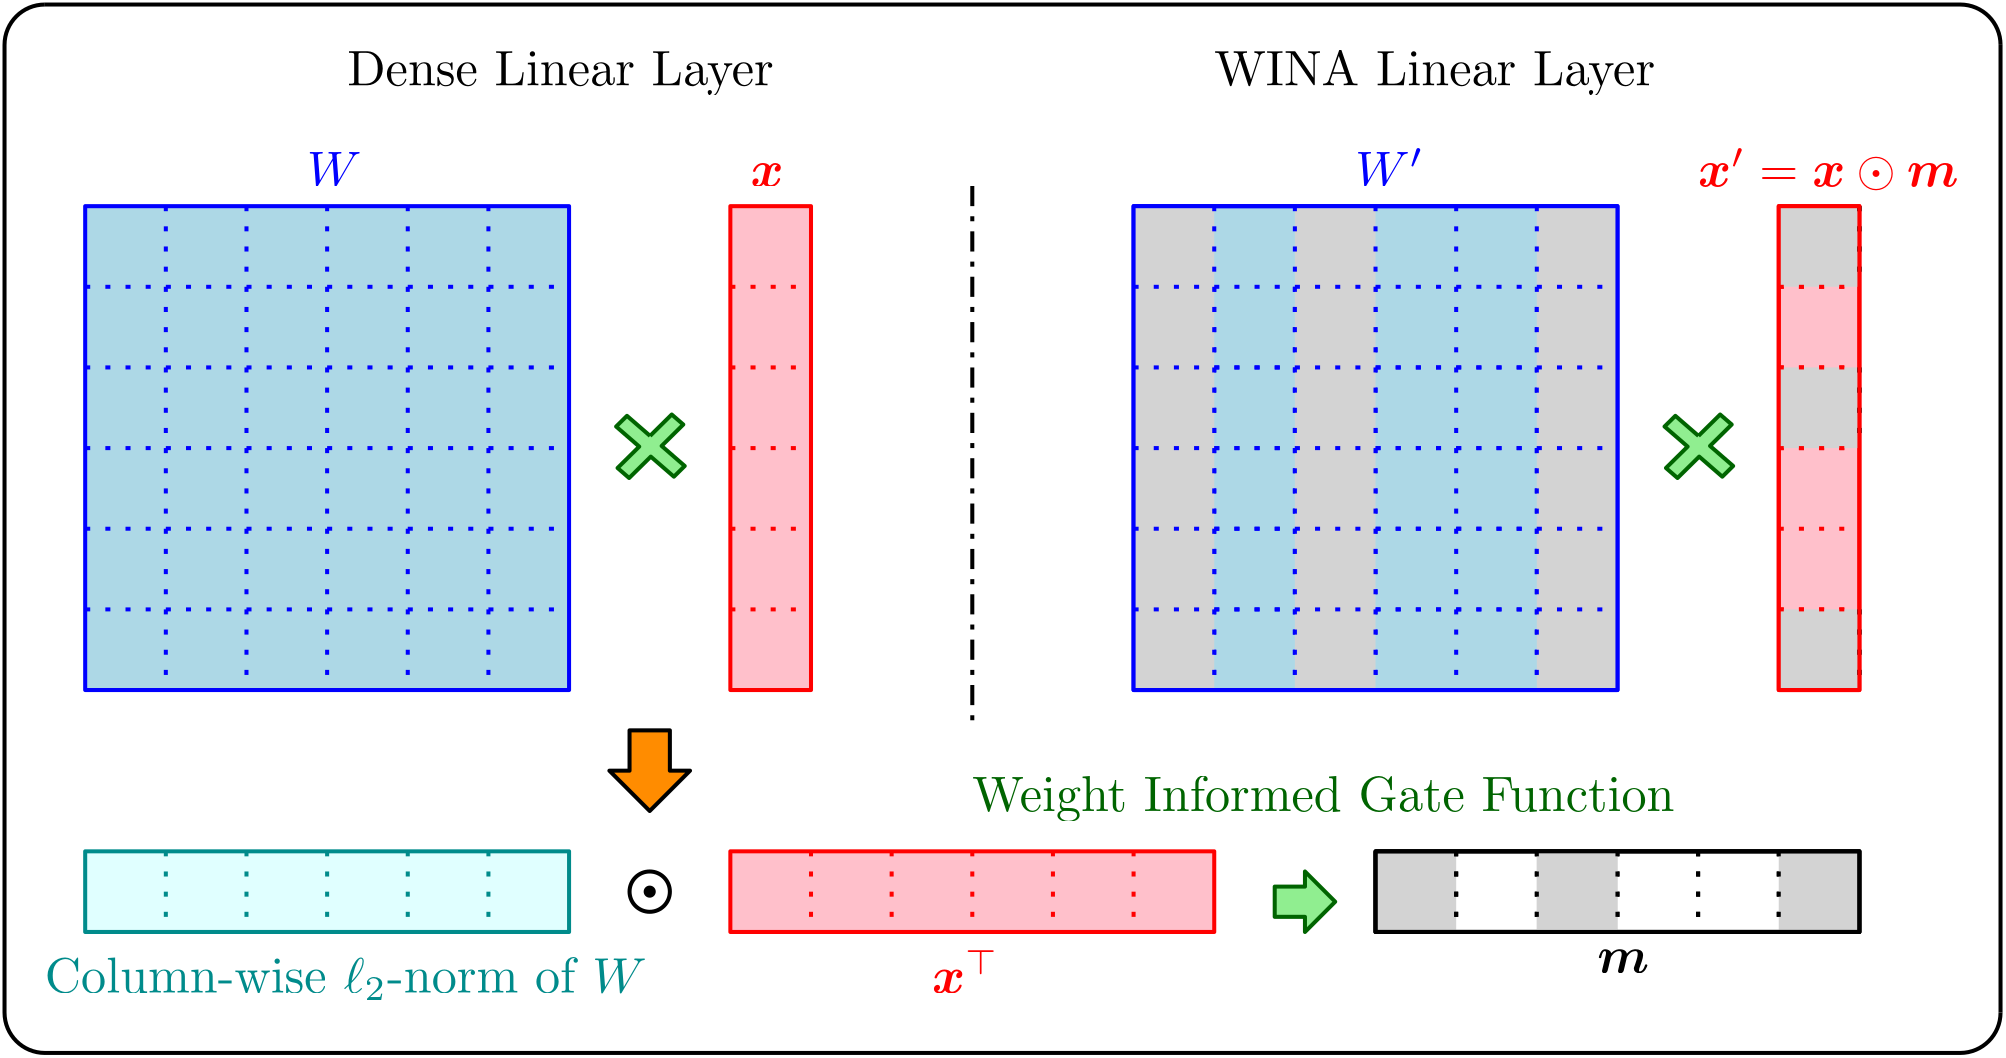
\includegraphics[width=0.8\textwidth]{overview.png}
	\caption{{\textbf{Overview of \algacro{}.} \algacro{} performs training-free sparse activation by selecting the most influential input dimensions based on both hidden state magnitudes and the column-wise $\ell_2$-norms of weight matrices. This joint criterion ensures accurate sub-network activation at each layer during inference, preserving model performance while reducing computational overhead.}}
	\label{fig:Overview}
\end{figure}

\subsection{Problem Statement}

{
	\textbf{Main Problem.}  
	Consider a deep neural network (DNN) $\mathcal{M}$ consisting of $L$ layers. We denote the weight matrix of the $l$-th layer as $W_l \in \mathbb{R}^{m_l \times n_l}$ and the corresponding input as an arbitrary tensor $X \in \mathbb{R}^{n_l \times s_l}$ for $l \in \{1, ..., L\}$, representing the full information content.  
	Our goal is to identify a set of binary activation gates $\mathcal{G} = \{\bm{g}_1, \cdots, \bm{g}_L\}$, where each $\bm{g}_l \in \{0, 1\}^{n_l}$, such that the deviation between the model's original output and the gated output is minimized:
	\begin{equation}
		\mathop{\text{minimize}}_{\bm{g}_1, \cdots, \bm{g}_L} \quad \norm{\mathcal{M}(X) - \mathcal{M}(X \mid \mathcal{G})}_2.
	\end{equation}
	
	Since obtaining the complete set of possible inputs $X$ is generally infeasible, we instead use a sampled subset $\tilde{X}$ to approximate it. The activation gating operates in the input vector space to reduce output deviation. With this observation, we can reformulate the original problem into a per-layer version to make the problem more tractable.
	
	\textbf{Refined Problem.}  
	Given a weight matrix $W \in \mathbb{R}^{m \times n}$ and a sampled input vector $\bm{x} \in \mathbb{R}^{n}$, the standard linear transformation is $\bm{y} \gets W \bm{x}$.  
	Our objective then becomes identifying an activation gate or mask $\bm{m} \in \{0, 1\}^{n}$ such that the masked output $\bm{y}_{\bm{m}} \gets W(\bm{m} \odot \bm{x})$ approximates the original by solving:
	\begin{equation}\label{main.prob}
		\mathop{\text{minimize}}_{\bm{m} \in \{0, 1\}^{n}} \quad  \norm{W \bm{x} - W(\bm{m} \odot \bm{x})}_2.
	\end{equation}
}

\subsection{Weight Informed Gate Function}

\textbf{Motivation.}
Many current sparse activation methods (\eg, Q-sparse~\citep{wang2024q}, CATS~\citep{lee2024catscontextuallyawarethresholdingsparsity}, TEAL~\citep{liu2024trainingfreeactivationsparsitylarge}) operate via a top-$K$ gating mechanism governed by the absolute values of the hidden states:
\begin{equation}
	\bm{m}_i = \begin{cases}
		1 & \text{if } |\bm{x}_i| \text{ is among the top-$K$ values in } |\bm{x}|, \\
		0 & \text{otherwise}
	\end{cases}
\end{equation}
However, this approach ignores the critical role that weight matrices play. Specifically, how each element of the preceding input interacts with the weight matrix $W$ in the forward propagation. This mismatch motivates us to propose \algacro{}, a method that jointly considers both inputs and weight matrices to minimize the approximation error for better performance.

\textbf{Formalization.}
In \algacro{}, we construct binary activation gates by selecting the top-$K$ components according to specific criteria:
\begin{equation}
	\bm{m}_i = \begin{cases}
		1 & \text{if } |\bm{x}_i \bm{c}_i| \text{ is among the top-$K$ values in } |\bm{x} \odot \bm{c}|, \\
		0 & \text{otherwise},
	\end{cases}
\end{equation}
where $\bm{c} \in \mathbb{R}^n$ represents the column-wise $\ell_2$ norm of $W$ and $\odot$ denotes the Hadamard or element-wise product.

The choice of $K$ can be adapted to different use cases, ranging from
(1) a coarse-grained universal criterion where a shared $K$ is applied across all layers to (2) a fine-grained layer-specific strategy that assigns $K$ individually to better minimize approximation error. 

% We provide pseudocode of \algacro{} in Algorithm \ref{alg:sparse_activation}. This algorithm performs sparse activation by selecting features based on the element-wise product of the absolute input values and the column-wise $\ell_2$ norms of the weight matrix. It supports two gating strategies: Top K (selecting the most important features of top k for each token) and Threshold (activating features throughout the batch by comparing the criterion values against a precomputed threshold determined by the sparsity level $s$). The gated (sparse) input is then projected using the weight matrix $W$ to produce the final layer output.


\begin{comment}
	\begin{algorithm}
		\caption{Sparse Activation via \algacro{}}
		\label{alg:sparse_activation}
		\begin{algorithmic}[1]
			\State \textbf{Input:} 
			\State \quad Input tensor $\bm{x}$.
			\State \quad Weight matrix $W \in \mathbb{R}^{m \times n}$,
			\State \quad Sparsity level $s \in [0,1)$\State \quad Gating method $\textit{strategy} \in \{\text{topk}, \text{threshold}\}$
			\State \textbf{Output:} 
			\State \quad Layer output tensor $y \in \mathbb{R}^{bs \times seq \times m}$
			\vspace{0.5em}
			\State \textcolor{gray}{\# Step 1: Compute column-wise $\ell_2$-norm of $W$}
			\State $a \gets \left[\left\|W_{:,i}\right\|_2\right]_{i=1}^{n}$ \quad \textcolor{gray}{$a \in \mathbb{R}^n$}
			\vspace{0.5em}
			\State \textcolor{gray}{\# Step 2: Compute activation criterion}
			\State $\hat{x} \gets |x|$ \quad \textcolor{gray}{$\hat x \in \mathbb{R}^{bs \times seq \times n}$}
			\State $h \gets \hat{x} \odot a$ \quad \textcolor{gray}{$h \in \mathbb{R}^{bs \times seq \times n}$}
			\vspace{0.5em}
			\State \textcolor{gray}{\# Step 3: Obtain input mask using Gating function}
			\State $g \gets \textsc{Gating}(h, s, \textit{strategy})$ \quad \textcolor{gray}{$g \in \{0,1\}^{bs \times seq \times n}$}
			\State $x' \gets g \odot x$
			\vspace{0.5em}
			\State \textcolor{gray}{\# Step 4: Get the layer output with sparse input}
			\State $y \gets x' W^{\top}$
			\vspace{0.5em}
			\Function{Gating}{$h, s, \textit{strategy}$}
			\If{$\textit{strategy} \text{ is topk}$}
			\State $k \gets \lfloor s \times n \rfloor$
			\State \textcolor{gray}{\# Top-k indices along feature dimension}
			\State $I \gets \text{TopkIndices}(h, k, \text{dim}=2)$ \quad \textcolor{gray}{$I \in \mathbb{R}^{bs \times seq \times k}$}
			\State 
			$\bm{g}_{i,j,t} = 
			\begin{cases} 1 & \text{if } t \in I_{i,j}, \\
				0 & \text{otherwise},
			\end{cases}$
			\ElsIf{$\textit{strategy} \text{ is threshold}$}
			\State \textcolor{gray}{\# Determine threshold based on $s$}
			\State $t_s \gets \textsc{ComputeThreshold}(h, s)$
			\State $g_{i,j,t} \gets \begin{cases}
				1 & \text{if } h_{i,j,t} > t_s \\
				0 & \text{otherwise}
			\end{cases}$
			\EndIf
			\State \Return $g$
			\EndFunction
		\end{algorithmic}
	\end{algorithm}
	
\end{comment}


\subsection{Theoretical Analysis}

{
	\algacro{} also offers theoretical advantages, capable of achieving a more optimal bound on the approximation error than TEAL. To demonstrate, we first present a Lemma for a single-layer network. 
	\begin{lemma}[Optimal approximation error over single layer]\label{lemma.single_layer}
		% \textcolor{black}{
			Let  $\bm{x} \in \mathbb{R}^n$ be an input vector and $W \in \mathbb{R}^{m \times n}$ be a matrix satisfying column-wise orthogonality: $W^\top W= I_{n}$ where $I_n$ is an identity matrix. For any target sparsity level $k \in \mathbb{N}^+$ satisfying $k < n$, the expected deviation
			between the original network output and the gated output via \textit{\algacro{}} is less or equal to that of \textit{TEAL}'s. Formally:  
			$$\mathbb{E}\left[ \| W\bm{x}_\text{\algacro{}} - W\bm{x} \|_2^2 \right] \le \mathbb{E}\left[ \| W\bm{x}_\text{TEAL} - Wx \|_2^2 \right],$$ 
			
			where $\bm{x}_\text{\algacro{}}$ is the sparse input via \algacro{}, retaining the $k$ elements activated with the largest $|x_j \cdot \|W_{\cdot,j}\|_2 |$, and $\bm{x}_\text{TEAL}$ is the sparse input via TEAL, retaining the $k$ elements with the largest $|x_j|$.
			% }
		
		\paragraph{Proof.} See Appendix.
		
	\end{lemma}
	
	Using our single-layer Lemma~\ref{lemma.single_layer}, we can extend it to $L$ linear layers. As stated in Theorem~\ref{thm.L_layers} below, we see that \algacro{} still achieves smaller approximation error than TEAL in the $L$ layer case.
	\begin{theorem}[Optimal approximation error over consecutive $L$ layer]\label{thm.L_layers}
		% \textcolor{black}{
			% Let variable $x \in \mathbb{R}^{d_0}$ be an input vector and $\{W^{(\ell)}\}_{\ell=1}^N$ be weight matrices for a $N$-layer neural network where each 
			% $W^{(\ell)} \in \mathbb{R}^{d_{\ell} \times d_{\ell-1}}$ satisfies column-wise orthogonality:
			% \begin{equation}
				% (W^{(\ell)})^\top W^{(\ell)} = I_{d_{\ell-1}}, \quad \forall \ell \in \{1,\ldots,N\}.
				% \end{equation}
			% For any target sparsity level $k \in \mathbb{N}^+$ satisfying $k < \min(d_{\ell})$, the expected deviation
			% between the original output and the gated output via \textit{\algacro{}} gating mechanism is less than or equal to that of \textit{TEAL} gating mechanism. Formally:
			% \begin{equation}\label{eq:sparse-error-bound}
				% \E\left[\left\|y_S^{(N)} - y\right\|_2^2\right] \leq 
				% \E\left[\left\|y_T^{(N)} - y\right\|_2^2\right],
				% \end{equation}
			% where $y_S^{(N)}$ and $y_T^{(N)}$ denote the final network outputs using \algacro{} and TEAL 
			% sparsification methods respectively, with $y = W^{(N)}W^{(N-1)}\cdots W^{(1)}\,x$ being the original dense output. 
			% }
		% \textcolor{black}{
			Let $\bm{x} \in \mathbb{R}^{d_0}$ be an input vector and $\{W^{(\ell)}\}_{\ell=1}^N$ denote the weight matrices of an $N$-layer neural network, where each $W^{(\ell)} \in \mathbb{R}^{d_\ell \times d_{\ell-1}}$. Suppose there exists a subset $\mathcal{S} \subseteq \{1,\ldots,N\}$ with $|\mathcal{S}| = k$ such that every matrix $W^{(\ell)}$ with $\ell \in \mathcal{S}$ is column-wise orthogonal, \ie, $(W^{(\ell)})^\top W^{(\ell)} = I_{d_{\ell-1}}$. For any target sparsity level $k \in \mathbb{N}^+$ with $k < \min_{\ell \in \{1,\ldots,N\}} d_\ell$, the expected deviation satisfies:
			\begin{equation}\label{eq:sparse-error-bound}
				\E\left[\left\|\bm{y}_\text{\algacro{}} - \bm{y}\right\|_2^2\right] \leq 
				\E\left[\left\|\bm{y}_\text{TEAL} - \bm{y}\right\|_2^2\right],
			\end{equation}
			where $\bm{y}_\text{\algacro{}}$ denotes the output produced by \textit{\algacro{}}; $\bm{y}_\text{TEAL}$ is the output of \textit{TEAL}; and $\bm{y}$ is the original dense network output without any sparsification.
			% }
	\end{theorem} 
	
	\paragraph{Proof.} See Appendix.
	
	Using these, we now consider realistic deep neural networks equipped with various activation functions. Our results remain valid for a large class of activation functions provided that they satisfy the monotonicity property (\eg, ReLU and several of its variants, sigmoidal and softmax, etc). Like before, we start with the simple single-layer case before extending to the multi-layer case. For completeness, we explicitly state the definition below.
	\begin{definition}[Monotonic increasing function (MIF)]
		A function $f: \mathbb{R} \to \mathbb{R}$ is \emph{monotonically increasing} if for any $x_1 \leq x_2$, then $f(x_1) \leq f(x_2)$.
	\end{definition}
	
	\begin{lemma}[Optimal approximation error over a single layer with MIF]\label{lemma:single_layer_act_function} 
		Let $\bm{x} \in \mathbb{R}^{n}$ be an input vector, $W \in \mathbb{R}^{m \times n}$ be a matrix that satisfies column-wise orthogonality, and $f: \mathbb{R} \to \mathbb{R}$ be an activation function that is a MIF. For any target sparsity level $k \in \mathbb{N}^+$ satisfying $k < n$, the expected deviation between the original output and the gated output via \textit{\algacro{}} gating mechanism is less than or equal to that of \textit{TEAL} gating mechanism. Formally: 
		$$\mathbb{E}\left[ \| f(W\bm{x}_\text{\algacro{}}) - f(W\bm{x}) \|_2^2 \right] \le \mathbb{E}\left[ \| f(W\bm{x}_\text{TEAL}) - f(W\bm{x}) \|_2^2 \right],$$ 
		where $\bm{x}_\text{\algacro{}}$ is the sparse input via \algacro{}, retaining the $k$ elements with the largest $|x_j \cdot \|W_{\cdot,j}\|_2 |$, and $\bm{x}_\text{TEAL}$ is the sparse input via TEAL, retaining the $k$ elements with the largest $|x_j|$.
	\end{lemma}
	
	\paragraph{Proof.} See Appendix.
	
	Finally, we extend this theorem to the case of a multi-layer network with MIF activations. 
	
	\begin{theorem}[Optimal approximation error over consecutive $L$ layer with MIF]  
		% \textcolor{black}{
			% Let variable $x \in \mathbb{R}^{d_0}$ be an input vector,  $\{W^{(\ell)}\}_{\ell=1}^N$ be weight matrices for a $N$-layer neural network where each 
			% $W^{(\ell)} \in \mathbb{R}^{d_{\ell} \times d_{\ell-1}}$ satisfies column-wise orthogonality, and $f: \mathbb{R} \to \mathbb{R}$ be an activation function with the Maximum Impact Property (MIF). For any target sparsity level $k \in \mathbb{N}^+$ satisfying $k < \min(d_{\ell})$, the expected deviation between the original output and the gated output via \textit{input-weight-based} gating mechanism (\textbf{\algacro{}}) is less than or equal to that of \textit{input-based} gating mechanism (\textbf{TEAL}). Formally:
			% \begin{equation}\label{eq:sparse-error-bound}
				% \E\left[\left\|y_S^{(N)} - y\right\|_2^2\right] \leq 
				% \E\left[\left\|y_T^{(N)} - y\right\|_2^2\right],
				% \end{equation}
			% where $y_S^{(N)}$ and $y_T^{(N)}$ denote the final network outputs using \algacro{} and TEAL 
			% sparsification methods respectively, with $y$ being the original dense output. 
			% }
		% \textcolor{black}{
			Let $\bm{x} \in \mathbb{R}^{d_0}$ be an input vector and $\{W^{(\ell)}\}_{\ell=1}^N$ denote the weight matrices of an $N$-layer neural network, where each $W^{(\ell)} \in \mathbb{R}^{d_\ell \times d_{\ell-1}}$. Suppose there exists a subset $\mathcal{S} \subseteq \{1,\ldots,N\}$ with $|\mathcal{S}| = k$ such that every matrix $W^{(\ell)}$ with $\ell \in \mathcal{S}$ is column-wise orthogonal, \ie, $(W^{(\ell)})^\top W^{(\ell)} = I_{d_{\ell-1}}$. Let $f: \mathbb{R} \to \mathbb{R}$ be an activation function satisfying the monotonic increasing property. For any target sparsity level $k \in \mathbb{N}^+$ with $k < \min_{\ell \in \{1,\ldots,N\}} d_\ell$, the expected deviation satisfies:
			\begin{equation}\label{eq:sparse-error-bound}
				\E\left[\left\|\bm{y}_\text{\algacro{}} - \bm{y}\right\|_2^2\right] \leq 
				\E\left[\left\|\bm{y}_\text{TEAL} - \bm{y}\right\|_2^2\right],
			\end{equation}
			where $\bm{y}_\text{\algacro{}}$ denotes the output produced by \textit{\algacro{}}; $\bm{y}_\text{TEAL}$ is the output of \textit{TEAL}; and $\bm{y}$ is the original dense network output without any sparsification.
			% }
	\end{theorem} 
}
\paragraph{Proof.} See Appendix.
% }
\paragraph{Remark.} Many commonly used activation functions are monotonically increasing, such as ReLU, LeakyReLU, etc., or nearly monotonically increasing, such as SiLU.  This fact largely ensures the generality of \algacro{} across a wide range of deep neural network architectures.

% \subsection{Practical Adaptation}
\subsection{From Theory to Practice}

\paragraph{Motivation.} In Section 3.3, our theoretical analysis relies on the assumption of column-wise orthogonality of the relevant weight matrices, i.e., $W^\top W = I$ when, in reality, LLMs can violate the column-wise orthogonality condition. To bridge this gap between theory and practice, while preserving the theoretical error bounds, we propose a tensor transformation framework that enforces column-orthogonality in the relevant weight matrices of the model.

\paragraph{Transformation Protocol.} Given a weight matrix $W$, we can enforce column-wise orthogonality by multiplying $W$ from the right by an orthogonal matrix $Q$ such that the product $WQ$ has orthogonal columns. Specifically, we perform Singular Value Decomposition (SVD) on $W$:
\[
W = U \Sigma V^\top
\]
where $U$ and $V$ are orthogonal matrices, and $\Sigma$ is a diagonal matrix containing the singular values of $W$. To achieve column-orthogonality, we set $Q = V$ and transform $W$ as follows:
\[
\hat W = W V
\]
This transformation guarantees that the resulting matrix $W'$ satisfies the column-orthogonality:
\begin{equation}
(\hat W)^\top \hat W = \Sigma^\top U^\top U \Sigma = \Sigma^2
\end{equation}

To ensure that the model's final output remains unchanged after this transformation, we compensate for its effects using computational invariance \citep{ashkboos2024slicegptcompresslargelanguage}; more specifically, we enforce column-wise orthogonality constraints on the key projection matrices $W_k$ in the self-attention layer and the gate projection matrices $W_{gate}$ in the MLP layer via SVD-based transformation. We then propagate these transformations through adjacent layers and adjust the residual connections accordingly to maintain computational invariance. During inference, we employ the proposed activation criterion on these transformed column-orthogonal matrices, while using the conventional input-based activation criterion for the remaining matrices as typically done in sparse modeling. 





% \subsection{Sparsification Function}
% \csh{
% Current sparse activation methods (e.g., TEAL) rely solely on the magnitude of hidden states to determine which elements to activate. However, the norms of the corresponding channels in the weight matrix also play a critical role. Some elements in the inputs may have small magnitudes but with large norms of the corresponding channel in the weight matrix. If we follow previous approaches that only activate elements with the largest magnitudes, these elements might be mistakenly deemed unimportant and zeroed out, leading to significant errors.

% Building upon this insight, our activation criteria must consider both the effect of hidden states and weight matrices. The key challenge lies in effectively combining these two factors. We aim to develop a strategy that satisfies: condition (1) yields smaller output errors compared to alternative approaches, and condition (2) comparable inference acceleration ability to alternative approaches.

% We have identified an activation criterion that satisfies the above conditions: the absolute value of the product between the inputs and the column-wise L2 norm of the weight matrix. We define the criterion $c_i$ for element $x_i$ as follows:}

% \begin{definition}[\jk{Definition for WHAT?}]
%     For a weight matrix $W \in \mathbb{R}^{m\times n}$ and vector $\bm{x}\in\mathbb{R}^n$, define activation criteria $c_i$ for element $x_i$ as follows:
%     $$c_i=|x_ia_i|$$

%     where $a \in \mathbb{R}^n$ is the column-wise L2 norm of $W$, the i-th element of $a$ is:
%     \[
%     a_j = \| W_{:,j} \|_2 = \sqrt{\sum_{i=1}^m W_{i,j}^2}
%     \]
% \end{definition}

% We then compute the threshold $t_p$ for a target sparsity level $p \in \left[ 0,1 \right ]$ based on the prior distribution of the criteria. $t_p$ satisfies:

% $$
% \frac{1}{n}\sum_{i=1}^{n}{P\left(\left| c_i \right| < t_p \right)}=p
% $$

% During inference, we compare the criterion value of input $x$ against the threshold and generate a corresponding mask $mask \in \mathbb{R}^n$ for $x$, where the i-th element of $mask$ is as follows:
% $$
% mask_{i} = \begin{cases} 
% 1, & \text{if } |c_i| > t_p \\
% 0, & \text{else}
% \end{cases}
% $$

% The input vector after sparsification function, $x'$ is:
% $$
% x' = x \odot mask
% $$

% \csh{
% In practice, we randomly select 1,000 samples from the Alpaca dataset to construct the input histogram and compute the threshold.

% This activation criterion satisfies two conditions mentioned above. 

% Regarding Condition (1), we rigorously demonstrate that under certain assumptions, our method outperforms input-only criteria across single-layer networks, multi-layer networks and multi-layer networks with activation functions. (Detailed proofs in Appendix A)

% For Condition (2), while our method requires computing $x·a$ during inference, this introduces negligible additional time cost because: (i) The column-wise L2 norms of the weight matrix $a$ are computed before inference. (ii) For $k$ tokens, the additional computation incurs $O(kn)$ time complexity. However, sparse activation reduces matrix multiplication costs by $O(pmKn)$, where $p$ is the sparsity ratio and $m$ the output dimension. Given typical configurations where $pm>>1$, this criterion has comparable inference acceleration ability to alternative approaches.
% }

% \subsection{Sparse-aware Distribution Constructions}

% \csh{
% TEAL construct histogram and calculate the threshold in a sparse-ignorant way.  Specifically, it constructs input histograms and computes activation thresholds under the assumption of a fully dense model, disregarding the cascading effects of sparse activation in earlier layers on subsequent layers inputs.

% \paragraph{Empirical Validation.} 
%  We empirically demonstrate that sparse activation induces significant input distribution shift. As shown in Figure 1, comparative analysis of the distribution of the final layer in Llama-3-8B reveals striking difference between the (1) Sparse-ignorant mode: input distributions constructed under full-density assumptions and (2) Sparse-aware Mode: distributions adapted to actual sparse activation.


% The observed distributional shift necessitates layer-adaptive distribution modeling. To address this, we use a sparse-aware distribution construction approach (Algorithm 1) that recursively adjusts input statistics based on sparse activations from preceding layers.
% }

% \begin{figure}
%   \centering
%   \includegraphics[width=\textwidth]{figures/distribution_comparison.png}
%   \caption{Comparison of the Input Distribution in the Final Layer of Llama-3-8B.}
% \end{figure}

% \begin{algorithm}
% \caption{Sparse-aware Activation Threshold Calculation}
% \label{alg:sparse_activation}
% \begin{algorithmic}[1]
	% \State \textbf{Input:} 
	% \State \quad Decoder layers $\{D_1, D_2, \ldots, D_L\}$,
	% \State \quad Input data $X \in \mathbb{R}^{b \times seq \times d}$
	% \State \quad sparsity parameters $\{s_l^{(i)}\}$ of the $i$-th linear layer in decoder layer $D_l$
	% \State \textbf{Output:} 
	% \State \quad Activation thresholds $\{t_l^{(i)}\}$ of the $i$-th linear layer in decoder layer $D_l$
	% \dz{we may need to edit this aglo to include the orthgonal transform, right?}
	% \For{each decoder layer $D_l\in \{D_1, D_2, \ldots, D_L\}$}
	%     \State \textcolor{gray}{\small \# Full forward pass to capture linear layer inputs}
	%     \State $O \leftarrow D^{full}_l(X)$
	%     \State $H^{(i)} \leftarrow$ input of the $i$-th linear layer in $D_l$
	%     \For{each linear layer $M^{(i)}$ with matrix $W^{(i)} \in \mathbb{R}^{b \times seq \times d^{(i)}_l}$ in $D_l$}
	%         \State \textcolor{gray}{\small \# Compute column-wise L2 norm of $W^{(i)}$}
	%         \State $a_j \leftarrow ||W^{(i)}_{:,j}||_2$
	%         \State \textcolor{gray}{\small \# Compute activation criterion of $M_i$}
	%         \State $\widehat{H}^{(i)} \gets H^{(i)} \cdot a$ 
	%         \State $\widehat{H}^{(i)}_j \gets |\widehat{H}^{(i)}_j|$
	%         \State \textcolor{gray}{\small \# Flatten and find top-$k$ threshold}
	%         \State $\widehat{H}^{(i)} \gets \text{flatten}(\widehat{H}^{(i)})$
	%         \State $k \gets \lfloor b \times seq \times d^{(i)}_l \times s_l^{(i)} \rfloor$
	%         \State $t_l^{(i)} \gets \text{top-}k(\widehat{H}^{(i)}, k) \quad \triangleright \text{Value of the $k_i$-th largest element}$
	%         \State Record $t_l^{(i)}$ for layer $D_l$
	%     \EndFor
	%     \State \textcolor{gray}{\small \# Sparse forward pass with calculated  thresholds to update hidden states}
	%     \State \quad $X \leftarrow D^{sparse}_l(X, \{t^{(i)}_{l}\})$
	% \EndFor
	% \State \Return $\{t_l^{(i)}\}$ for all $l, i$
	% \end{algorithmic}
% \end{algorithm}

% \begin{algorithm}
% \caption{Sparse-aware distribution construction}\label{alg:cap}
% \begin{algorithmic}
	% \Require $X \in \mathbb{R}^{B \times \ seq \times d}$, $n$ Layers, $m$ matrices and projections for each layer, step size $\beta$ \\
	% \dz{@Sihan: you should structure this algorithm to be a bit more clear especially since this is one of the core points of the paper -- reviewers will look it over for about 30 sec and will either get a good/bad impression. Bad impression is likely if things aren't clear from the first glance.
		
		% You should have a \textbf{Input(s):} and \textbf{Output(s):} instead of \textbf{Require:} at the very beginning.
		% Also, some of the variables I think will be confusing to the reviewers especially those who aren't already familiar with this. Spell everything out! For example, 
		
		% 1) What's $M_{i,j}$? 
		
		% 2) What variables are the projections? Is $W$ the weights? How is $W$ different from $M$?
		
		% 3) Difference between weight matrices and and projections?
		
		% Also some inconsistencies are present: e.g., you define $X$ as input but then refer to $x$ instead
		% }
	
	% \State \#Construct inputs distribution independently
	% \For{$i = 1,\dots,n$}
	%     \For{$j = 1,\dots,m$}
	%         \State $a_{i,j} \gets norm(W_{i,j})$ \# get column-wise L2 norm of matrices $M_{i,j}$
	%         \State $s \gets x \odot a_{i,j}$ \dz{Is this missing a step? Is}
	%         \State $D_{i,j} \gets distribution(s)$ \dz{What's the distribution operator? This algorithm should be self-contained so that if the reader just looks at this table for Algorithm 1 without reading much of the text, they should still know what you're doing}
	%         \State $x=J_{i,j}(x)$ \# Forward pass through projection $J_{i,j}$
	%         \State Record $D_{i,j}$
	%     \EndFor
	% \EndFor
	% \State \#Block-wise greedy optimization
	% \State $f_j \gets size(W_j)$ for $j=1,\dots,m$ \dz{define what size is explicilty or in comments (with \#)}
	% \State $F \gets \sum_{j=1}^{m}{f_j}$
	
	% \For{$i = 1,\dots,L$}
	%     \State $p \gets 0$, $P \gets 0$
	%     \While{$P<1$}
	%         \For{$j = 1,\dots,m$}
	%             \State $p_{i,j}+=\beta\cdot (F/f_{j})$
	%             \State $t_{i,j} \gets threshold(D_{i,j}, p_{i,j})$ 
	%             \State $E_{i,j} \gets ||Y_{gt}-J(X,t_{i,j})||_{2}$
	%             \State $p_{i,j}-=\beta\cdot (F/f_{j})$
	%         \EndFor
	%         \State $t \gets argmin_tE_{i,t}$
	%         \State $p_{i,t}+=\beta\cdot (F/f_{t})$
	%         \State $P = \sum_{j=1}^{m}{p_{i,j}\cdot f_j}/F$
	%     \EndWhile
	% \EndFor
	% \State \#Construct inputs distribution layer-wise dependently
	% \For{$i = 1,\dots,n$}
	%     \For{$j = 1,\dots,m$}
	%         \State $s \gets x \odot a_{i,j}$
	%         \State $D_{i,j} \gets distribution(s)$
	%         \State $p \gets p_{i,j}$ 
	%         \State $t_{i,j} \gets threshold(D_{i,j}, p)$ \# set threshold for projection $J_{i,j}$
	%         \State $x=J_{i,j}(x,t_{i,j})$
	%     \EndFor
	% \EndFor
	% \end{algorithmic}
% \end{algorithm}